\chapter{Class 16}
\begin{theorem}[Soundness] If $\{\phi\} \vdash \{\psi\}$ then $\{\phi\} \models\{\psi\}$ such that for 
    \begin{itemize}
        \item partial correctness programs we have that
        \[
            \forall \sigma\sigma'  \forall I, ~ \sigma \models^I \phi \land \langle c,\sigma\rangle\downarrow \sigma' \Rightarrow \sigma' \models^I \psi,  
        \]
        \item and for total correctness programs we have that
        \[
            \forall \sigma \forall I, ~ \sigma \models^I\phi \Rightarrow \exists \sigma', \langle c, \sigma \rangle\downarrow\sigma' \land \sigma'\models^I \psi.    
        \]
    \end{itemize}
\end{theorem}


\begin{theorem}[Relative Completeness] We have an oracle for deciding $\models \chi$ (the validity of assertions), if $\models \{\phi\} c \{\psi\}$ then $\vdash \{\phi\} c \{\psi\}$.
    \label{thm:relative-completeness}
\end{theorem}

However, the following issues arise:
\begin{itemize}
    \item $\models \{true\} c \{false\}$ \texttt{iff} c does not terminate.
    \item $\models \{true\} skip \{\psi\}$ \texttt{iff} $\models \psi$, but according to G\"{o}del theorem there is no complete proof system for $(\mathbb{N}, +, \times)$.
\end{itemize}

\section{Verification Conditions}
In general, we can derive verification conditions using the following rules:
\begin{itemize}
    \item $vc(\{\phi\} skip \{\psi\}) = \{\phi \Rightarrow \psi\}$.
    \item $vc(\{\phi\} x=a \{\psi\}) = \{\phi \Rightarrow \psi_{[x \mapsto a]}\}$.
    \item $vc(\{\phi\} c_1 \{\chi\} c_2 \{\psi\}) = vc(\{\phi\} c_1 \{\chi\}) \cup vc(\{\chi\} c_2 \{\psi\})$.
    \item $vc(\{\phi\} \texttt{if }b \texttt{ then } c_1 \texttt{ else }c_2 \{\psi\}) = vc(\{\phi\land b\} c_1 \{\psi\}) \cup vc(\{\phi \land \neg b\} c_2 \{\psi\})$.
    \item $vc(\{\phi\} \texttt{ while } \{\chi\} ~b \texttt{ do } c \{\psi\}) = \{\phi \Rightarrow \chi, \chi \land \neg b \Rightarrow \psi\} \cup vc(\{\chi \land b\} c \{\chi\})$.
\end{itemize}
\subsection{Annotated Program}
\begin{algorithm}[!h]
    \caption{A program that computes $m\times n$}\label{alg:cap}
    \begin{algorithmic}
    \State $\{true\}$
    \State $x \coloneqq 0$
    \State $\{x=0\}$
    \State $y \coloneqq 0$
    \State $\{x=0 \land y=0\}$
    \While{$y \leq n$} \Comment{loop invariant: $\{x=m\times y \land y\leq n\}$}
        \State $\{x = m\times y \land y < n\}$
        \State $x \coloneqq x + m$
        \State $\{x = m\times (y+1) \land y < n\}$
        \State $y \coloneqq y + 1$
    \EndWhile
    \State $\{x = m\times n\}$
    \end{algorithmic}
\end{algorithm}

From the annotations shown in Algorithm \ref{alg:cap} we can derive the verification conditions which are the assertions that need to be valid for the Hoare proof:
\begin{itemize}
    \item $true \Rightarrow 0 = 0$.
    \item $x=0 \Rightarrow x=0 \land 0=0$.
    \item $x=0 \land y=0 \Rightarrow x=m\times y \land y \leq n$.
    \item $x=m\times y \land y \leq n \land y \geq n \Rightarrow x=m\times n$.
    \item $x=m\times y \land y \leq n \land y < n \Rightarrow x=m\times y \land y < n$.
    \item $x=m\times y \land y < n \Rightarrow x + m=m\times (y+1) \land y < n$.
    \item $x= m\times(y+1) \land y < n \Rightarrow x = m\times (y+1) \land (y+1) \leq n$.
\end{itemize}

\subsection{Flow Chart (Control Flow Graph - ``Floyd Style")}
    The annotations for the same example can be seen in Figure \ref{cf16}.
\begin{figure*}[h!]
    \begin{center}
    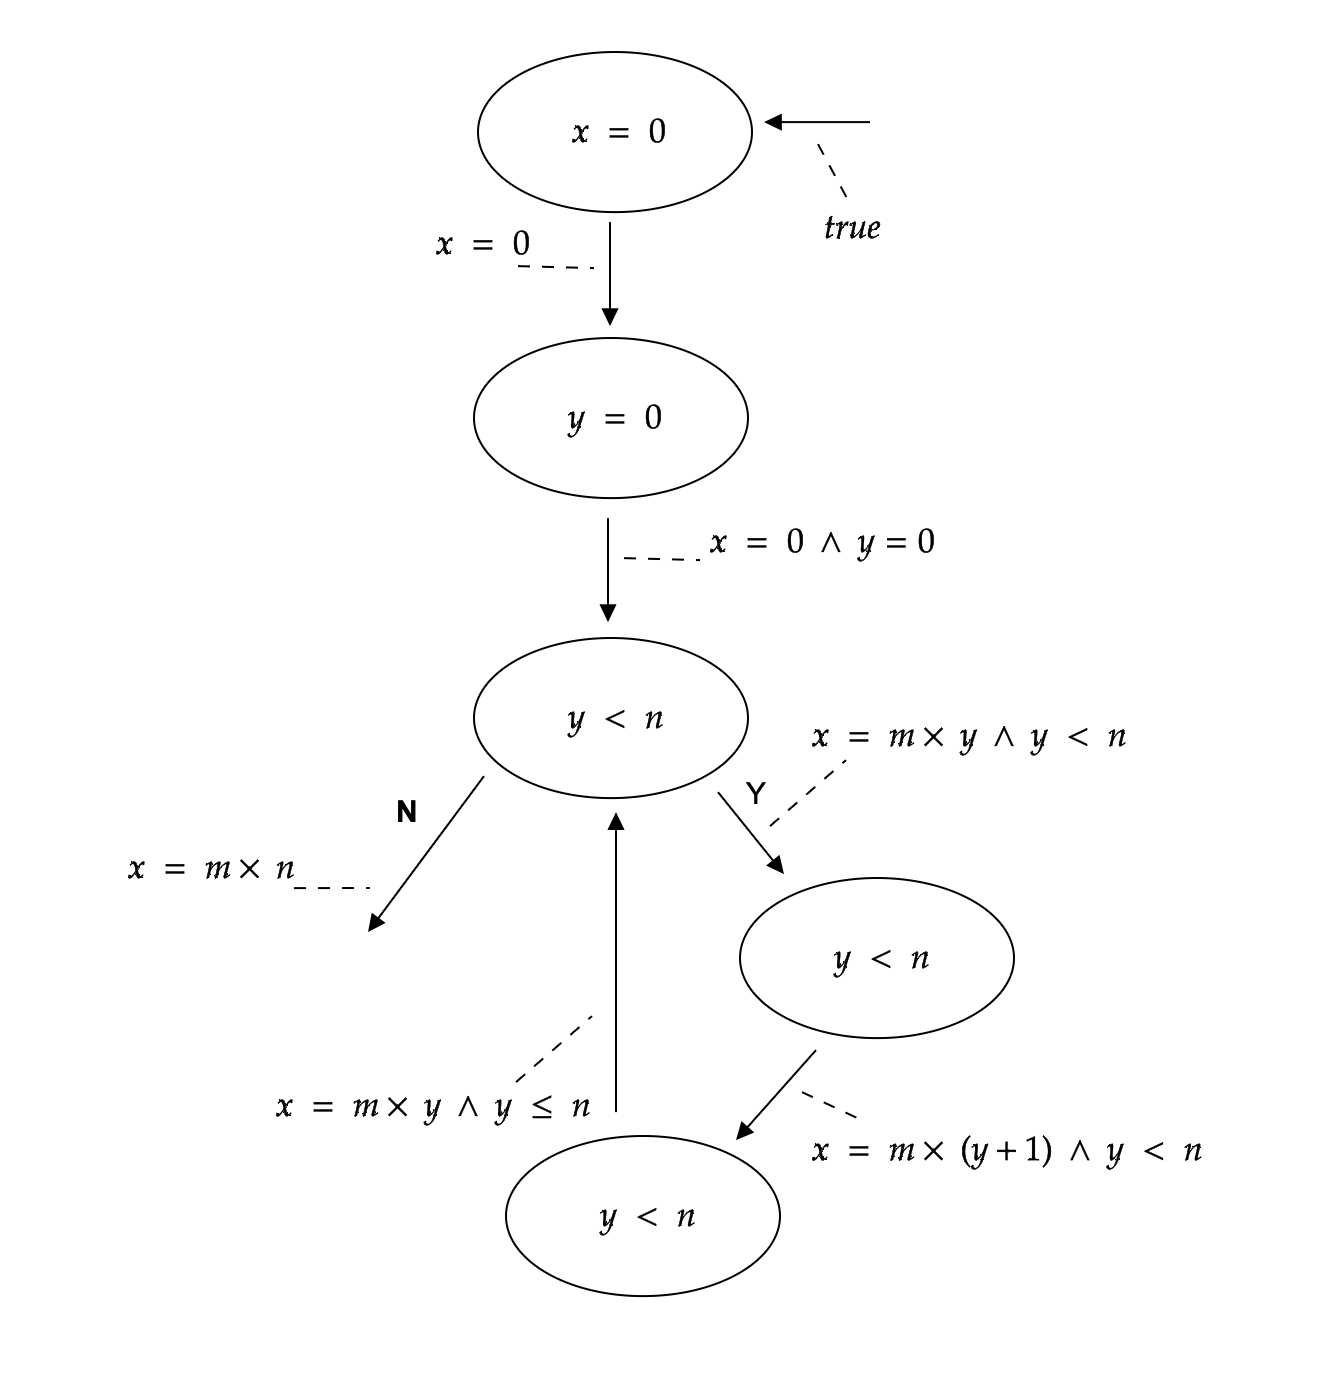
\includegraphics[width=\linewidth]{images/cf16.png}
    \caption{Control flow graph of the program that computes $x = m \times n$.}
    \end{center}
    \label{cf16}
\end{figure*}

\pagebreak

\section{Programs as predicate transforming (Dijkstra): Weakest (liberal) preconditions}
\begin{definition}[Weakest Liberal Preconditions] $wlp(c, \psi)$ is the \textit{weakest} $\phi$ s.t $\{\phi\} c \{\psi\}$ (for all $\phi$ with $\{\phi\} c\{\psi\}, \phi \Rightarrow wlp(c, \psi)$).
\end{definition}

\begin{definition}[Weakest Preconditions] $wp(c, \psi)$ is the \textit{weakest} $\phi$ s.t $\{\phi\} c \{\psi\} \land \forall \sigma,$ if $\sigma \models \phi$ then c terminates from $\sigma$.
\end{definition}


An assertion language is \underline{expressive} if $wlp(c,\psi) = \{\sigma \in \Sigma \mid \langle c, \sigma\rangle = \bot \lor \forall I. \llbracket c \rrbracket \sigma \models^I\psi\}$.

For IMP, arithmetic $(\mathbb{N}, +, \times)$ is expressive (proof by G\"{o}delization of program executions).

\begin{example} 
    \begin{itemize}
        \item $wlp(skip, \psi) = \psi$
        \item $wlp(x=a, \psi) = \psi_{[x\mapsto a]}$
        \item $wlp(c_1, c_2, \psi) = wlp(c_1, wlp(c_2, \psi))$
        \item $wlp(\texttt{if } b \texttt{ then } c_1 \texttt{ else } c_2, \psi) = (b\Rightarrow wlp(c_1, \psi)) \land (\neg b \Rightarrow wlp(c_2, \psi)) = (b \land wlp(c_1, \psi)) \lor (\neg b \land wlp(c_2, \psi))$.
        \item $wlp(\texttt{while } b \texttt{ do } c, \psi) = \texttt{weakest }\chi$ s.t 1) $\chi \land b \Rightarrow wlp(c, \chi)$ and 2) $\chi \land \neg b \Rightarrow \psi$.
        \item For a fresh variable $n$, $wp(\texttt{while } b \texttt{ do } c, \psi) = \texttt{weakest }\chi$ s.t for a fresh variable $n$ 1) $\chi \land b \land e = n \Rightarrow wlp(c, \chi \land e > n)$, 2) $\chi \land \neg b \Rightarrow \psi$, and 3) $\chi \Rightarrow e \in $ well founded set.
    \end{itemize}
    
\end{example}

